\documentclass[border=10pt]{standalone}
\usepackage{pgfplots}
\pgfplotsset{compat=1.18}
\begin{document}
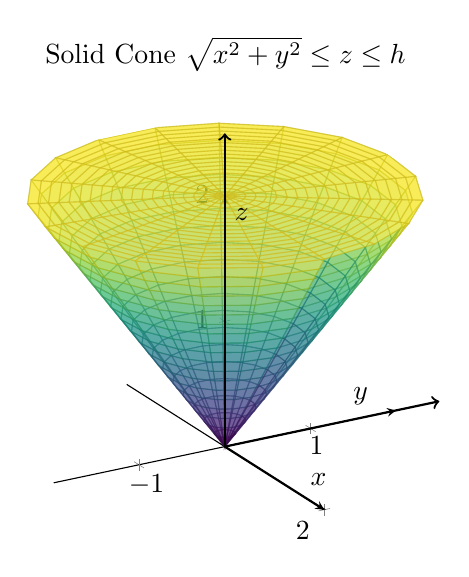
\begin{tikzpicture}
\begin{axis}[
    view={60}{30},
    xlabel={$x$},
    ylabel={$y$},
    zlabel={$z$},
    axis lines=center,
    colormap/viridis,
    title={Solid Cone $\sqrt{x^2+y^2} \leq z \leq h$}
]
    % Drawing the cone side
    \addplot3[surf, domain=0:2, y domain=0:2*pi, samples=20, opacity=0.5, colormap/viridis] 
    ({x*cos(deg(y))}, {x*sin(deg(y))}, {x});
    
    % Drawing the top cap
    \addplot3[surf, domain=0:2, y domain=0:2*pi, samples=20, opacity=0.5, colormap/viridis] 
    ({x*cos(deg(y))}, {x*sin(deg(y))}, {2});

    % Axis markers
    \draw[->, thick] (axis cs:0,0,0) -- (axis cs:2.5,0,0);
    \draw[->, thick] (axis cs:0,0,0) -- (axis cs:0,2.5,0);
    \draw[->, thick] (axis cs:0,0,0) -- (axis cs:0,0,2.5);
\end{axis}
\end{tikzpicture}
\end{document}
